\subsubsection{Infinite Horizon}
\begin{frame}{\subsecname: \subsubsecname}
    \begin{figure}
        \centering
        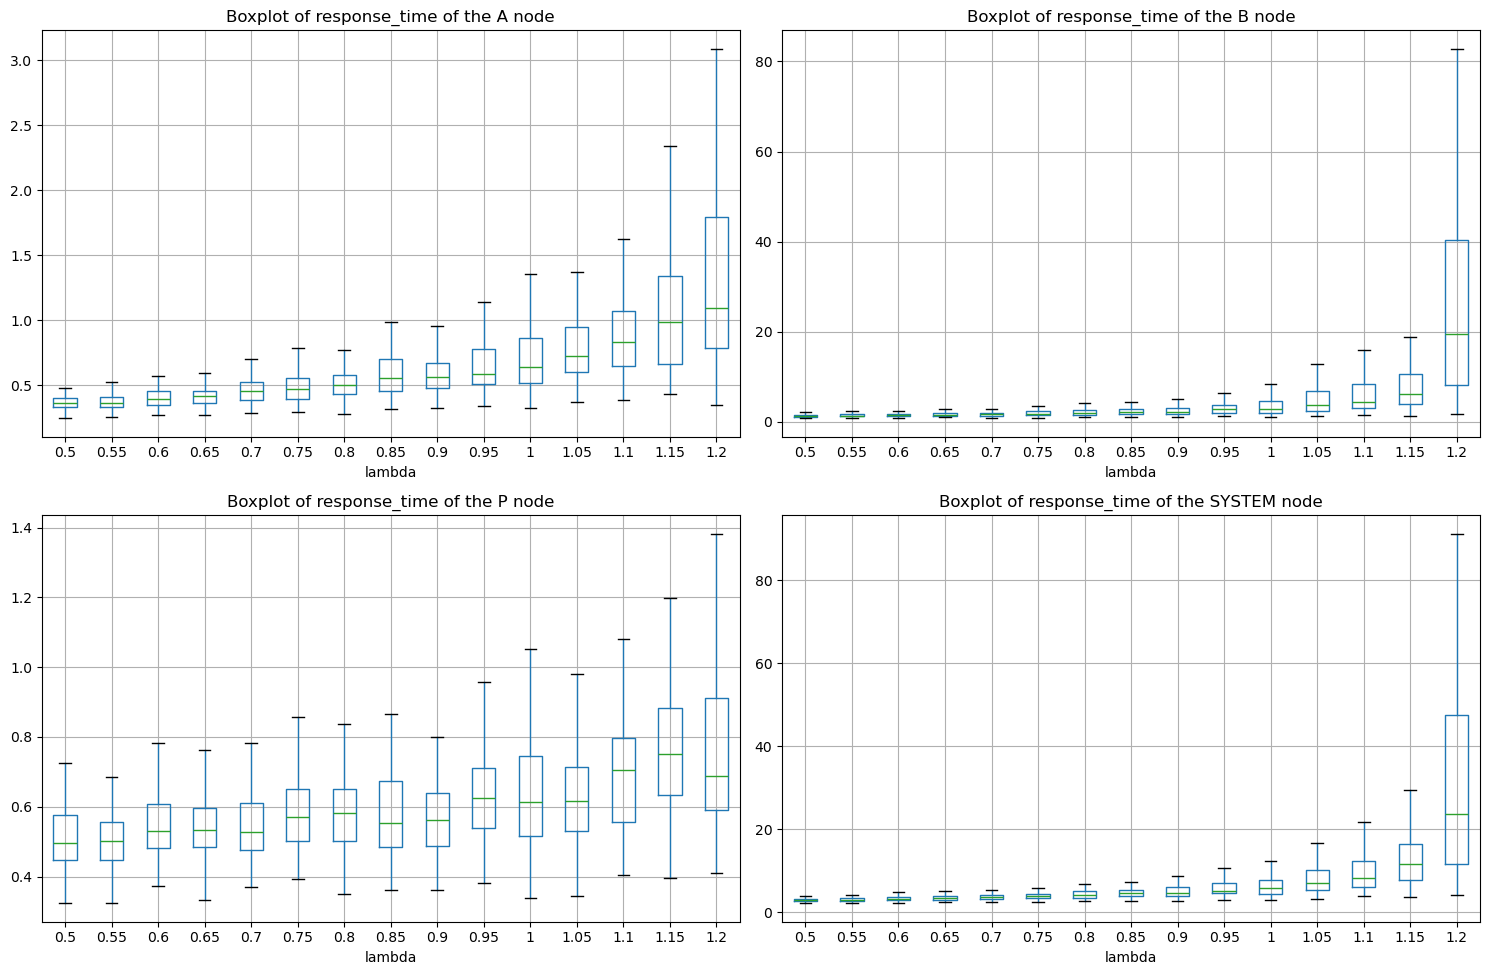
\includegraphics[width=0.75\linewidth]{figs/results/obj1/obj1-box-response-time.png}
        \caption{Distribuzione del Tempo di Risposta medio dei risultati sperimentali dell’obbiettivo 1}
        \label{fig:enter-label}
    \end{figure}
\end{frame}

\subsubsection{Finite Horizon}
\begin{frame}{\subsecname: \subsubsecname}
    \begin{figure}
        \centering
        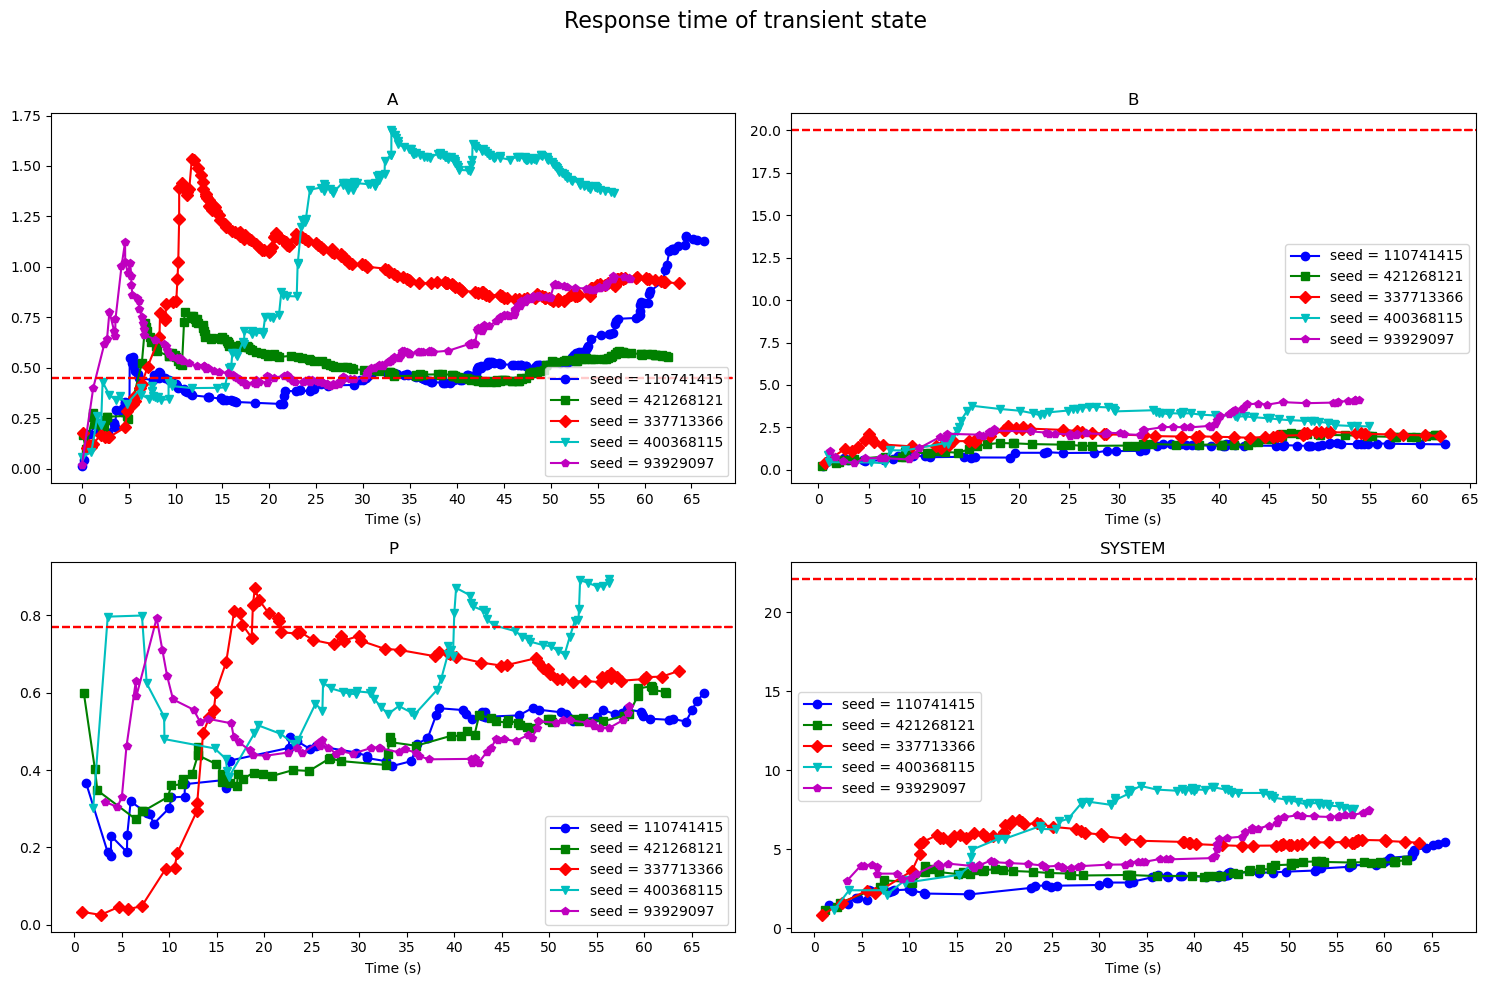
\includegraphics[width=0.75\linewidth]{figs/appendices/transient/obj1-transient-rtime-analitycal.png}
        \caption{Tempo di risposta per l’obiettivo 1 in funzione del tempo di simulazione nello stato transiente del sistema con un rate di arrivi 1.2 $job/s$ al variare del seed}
        \label{fig:enter-label}
    \end{figure}
\end{frame}

\subsubsection{Verification}
\begin{frame}{\subsecname: \subsubsecname}
\begin{figure}
    \centering
    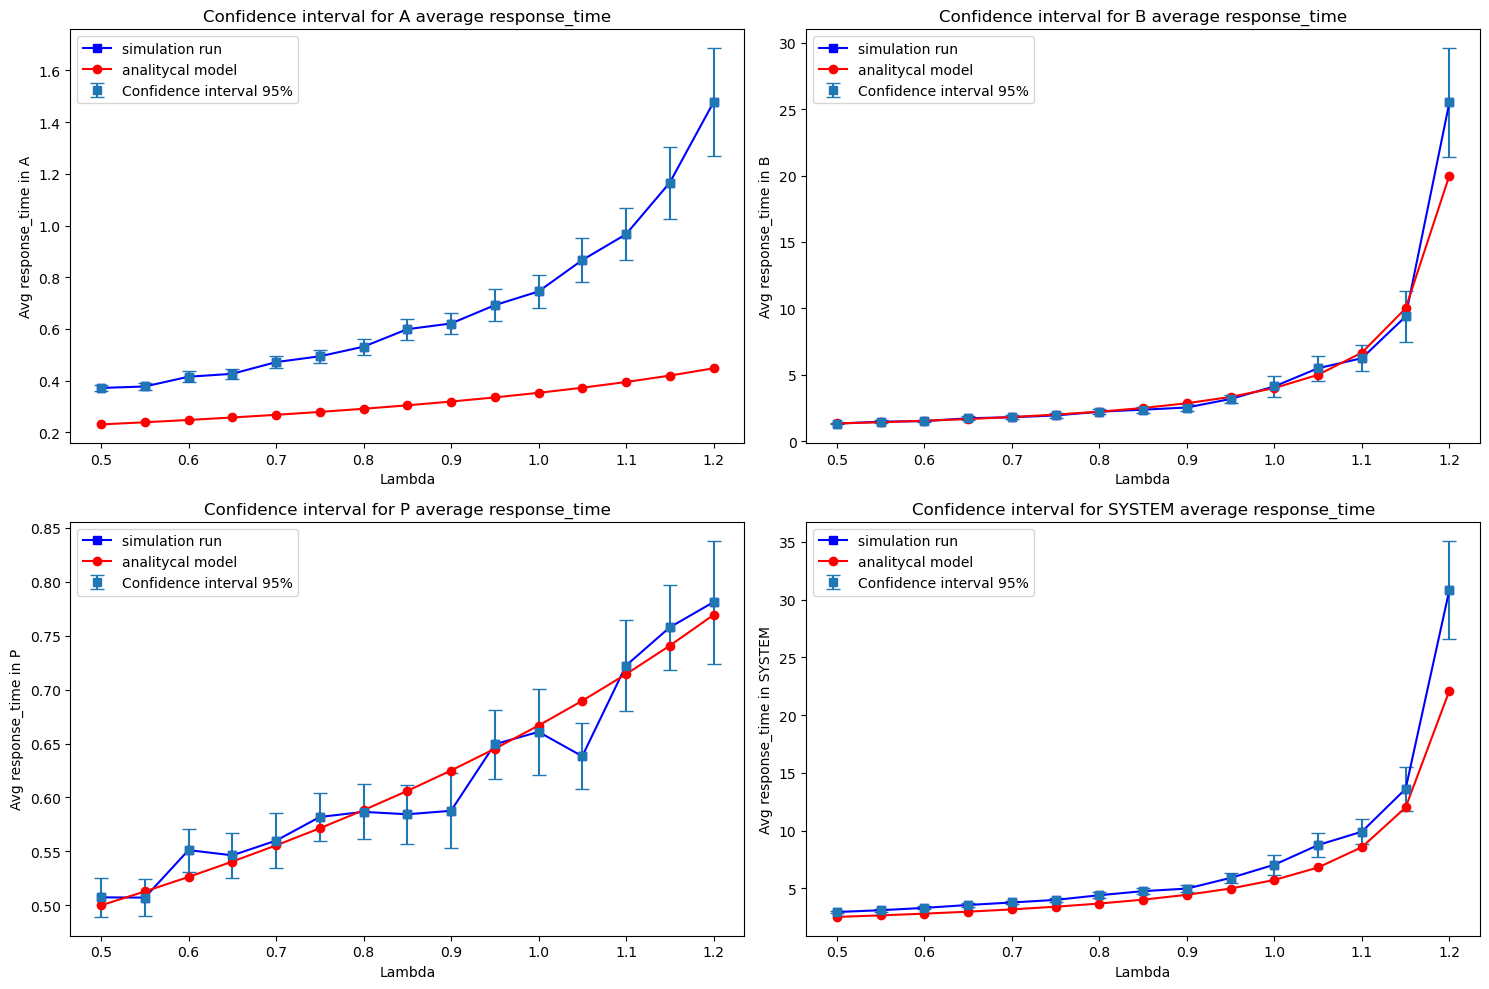
\includegraphics[width=0.75\linewidth]{figs/results/obj1/obj1-line-response-time.png}
    \caption{ Confronto tra valori medi della simulazione e del modello analitico del Tempo di Risposta per l’Obiettivo 1.}
    \label{fig:enter-label}
\end{figure}   
\end{frame}